\documentclass{CUP-JNL-PHO}%

\usepackage{libertine} 
%%%% Packages
\usepackage{graphicx}
\usepackage{multicol,multirow}
\usepackage{amsmath,amssymb,amsfonts}
\usepackage{mathrsfs}
\usepackage{amsthm}
\usepackage[figuresright]{rotating}
\usepackage{appendix}
\usepackage[authoryear]{natbib}
\usepackage{ifpdf}
\usepackage[T1]{fontenc}
\usepackage{newtxtext}
\usepackage{newtxmath}
\usepackage{textcomp}
\usepackage{xcolor}
\usepackage{tabularx}
\usepackage[colorlinks,allcolors=blue]{hyperref}

\newtheorem{theorem}{Theorem}[section]
\newtheorem{lemma}[theorem]{Lemma}
\theoremstyle{definition}
\newtheorem{remark}[theorem]{Remark}
\newtheorem{example}[theorem]{Example}
\numberwithin{equation}{section}

\articletype{ARTICLE}
%\artid{20}
\jyear{2020}
%\jvol{4}
%\jissue{1}
\jdoi{10.1017/S0373463320000247}
%\raggedbottom


% Han's packages
\usepackage{phonrule}
\usepackage{booktabs}
\usepackage{tipa}
\usepackage{tikz}
\usetikzlibrary{arrows, arrows.meta, positioning, matrix, tikzmark,calc, automata}
\usepackage{subcaption}
\theoremstyle{definition}
\newtheorem{definition}{Definition}[section]


\newcommand{\hijeff}[1]{\textcolor{red}{\textbf{[#1]}}}
\newcommand{\kuo}[1]{(\ref{#1})}










\begin{document}

\begin{Frontmatter}

\title{Learning Tonotactic Patterns with Autosegmental Representations}

\author[]{Han Li}
\author[]{Jeffrey Heinz}

\authormark{Li \& Heinz}

\address[]{\orgname{Department of Linguistics},
	\orgaddress{Stony Brook University},
	\postcode{Stony Brook, NY},
	\country{USA},
	\email{han.li.4/jeffrey.heinz@stonybrook.edu}}


\received{28 August 2025}
\accepted{31 May 2026}
	

\keywords{autosegmental representation, tonotactic learning, Hausa, tonal language}


\abstract{This paper presents and evaluates an algorithm which learns
	tonotactic patterns over autosegmental representations (ARs),
	facilitated in part by showing how adjacency matrix representations can represent ARs. The Bottom-Up Factor Inference Algorithm over ARs (BUFIA-AR) takes AR
	graphs as input, and outputs a set of inviolable subgraphs as
	constraints. The input AR graphs themselves are generated
	automatically from linear transcriptions.
	A corpus of 621 non-derived native Hausa words was used to test
	BUFIA-AR, which returned 11 constraints. The results fall into three
	categories: constraints that align with previous generalisations,
	constraints that provide more specific generalisations than
	previously posited and which better account for the data, and
	constraints that identify novel patterns. These results demonstrate
	the feasibility and efficiency of ARs as a computational
	representation for phonotactic learning.}

\end{Frontmatter}

\tableofcontents

\section{Introduction}\label{sec:intro} 
This paper provides one
method for learning tonotactic patterns over autosegmental
representations (ARs). A key insight of phonological theory is to view
forms in tonal languages as \textit{autosegmental graphs}, rather than
one-dimensional linear strings \citep{goldsmith1976autosegmental,
	coleman1991no, jardine2017LocalNature,
	oakdenNotationalEquivalenceTonal2020}. These representations have
been argued to have demonstrated advantages for analysing tonal
patterns \citep{hyman2009representation, clements2010autosegmental,
	oddenintroducing2013}.  Computationally, grammars over ARs have been
shown to express both local and long-distance constraints, while
maintaining a relatively low level of computational complexity
\citep{jardine2017LocalNature, chandleejardine19aisl}.  However,
despite the importance of ARs in tonal phonology and previous research
on their formal properties \citep{kornai2007mathematical}, there has
been limited work on learning tonal grammars, and no phonotactic
learning models to our knowledge have adopted ARs.

This paper focuses on learning tonotactic grammars. Following
\citet{jardine2017LocalNature}, the tonotactic grammar consists of a
set of language-specific inviolable constraints over ARs. The
constraints themselves only specify marked AR structures. Logically,
such grammars are simply the conjunction of negative literals
\citep{rogers.lambert2019mol}. In this setting, the tonotactic
learning problem boils down to identifying those constraints (the
marked AR structures) which are consistent with the entire dataset.

The Bottom-Up Factor Inference Algorithm (BUFIA) is a learning
algorithm that deterministically searches a space of possible
constraints and is provably guaranteed to find the most general
constraints consistent with its input data \citep{chandleeBufia2019,
	rawski2021structure}. Crucially, it is couched in model theory
\citep{Rogers1998, enderton2001mathematical} so that it can operate
with any particular representational scheme.

This work presents BUFIA-AR, an instantiation of BUFIA that learns
tonotactic constraints expressed with ARs. As will be explained, this
implementation utilises a matrix-based representation for ARs, which
is an adaptation of matrix-based representations of graphs
\citep{west2001introduction,CLRS2022}.

BUFIA-AR was tested on a curated corpus of Hausa \citep{wold-4}, a
Chadic language in West Africa. The corpus consists of 621
mono-morphemic words, which altogether provides a collection of 64
distinct ARs.  Using this corpus as input, we assess the performance
of BUFIA-AR through a combination of qualitative and quantitative
evaluations. Qualitatively, BUFIA-AR returns a grammar
consisting of 11 AR constraints when syllable, tone, and mora counts
are limited to three. These BUFIA-AR-learned constraints either align
with, or are more specific than, those previously proposed in the
literature. The algorithm additionally identifies novel patterns that
have not been previously reported. Quantitatively, a cross-validation
experiment shows that BUFIA-AR achieves a mean accuracy over 90\% in
both token- and type-based settings which outperforms the linguistic 
baseline grammar and a BUFIA learner using
string representations (BUFIA-Str). Altogether, these results
demonstrate the feasibility of using BUFIA-AR for tonotactic grammar
inference. All data and programs used in this paper are accessible on
GitHub.

In this way, this paper takes a first step towards learning tonal
grammars expressed in terms of ARs. We acknowledge that tonal grammars
are much more than just the tonotactic component. The grammars that
BUFIA-AR returns have nothing to say about how underlying
representations of tonal languages are learned, nor how these
underlying representations are transformed into surface
representations. We also acknowledge that some surface constraints
have been argued to follow from the tonal processes themselves in some
languages (see Section~\ref{sec:learning}), which is again something
the grammars returned by BUFIA-AR cannot express. Nonetheless, despite
these limitations, BUFIA-AR still makes a contribution to our
understanding of how tonal grammars expressed in terms of ARs can be
learned. We expect that some of the insights made here will persist in
future research which addresses these broader problems regarding the
learning of tonal grammars.

This paper is structured as follows. Section~\ref{sec:learning}
provides an overview of the tonotactic learning problem and current models. Section~\ref{sec:prelim} introduces 
formal language theory, model theory, and graph theory relevant to ARs
and BUFIA. Section~\ref{sec:bufiaar} provides a detailed description
of the BUFIA-AR implementation. Section~\ref{sec:hausa} presents the Hausa case study and model evaluation. Section~\ref{sec:discussion}
discusses issues relating to constraint optimisation, constraint
satisfaction, and constraint weighting. Section~\ref{sec:conclusion}
concludes the paper and points to some future directions.


\section{Learning Tonotactics} \label{sec:learning}
\subsection{Tonal Mapping Problem}\label{sec:learning.mapping}

A central question in tonal phonology concerns how languages organise 
tones, syllables, and/or moras into well-formed structures. A 
closely related modelling question asks what kinds of well-formed 
tonal patterns are attested in a language, and how such patterns 
can be systematically characterised. To illustrate these issues, 
we begin with a frequently discussed example: the tonal mapping 
problem in two West African tonal languages, Hausa and Mende. 
Hausa is a Chadic language, while Mende is a Southwestern Mande 
language spoken in Sierra Leone \citep{lebenRepresentationTone1978}.
Both languages use High (H) and
Low (L) tones as basic tonemes with the mora as the tone bearing unit
(TBU). However, they show distinct patterns in how their tonal
melodies are mapped to TBUs \citep{Newmanbook,
	lebenRepresentationTone1978, zoll2003optimal, jardine2017LocalNature}.  

  
As shown in Table~\ref{tab.hausa.mende}, the two languages first differ in their
monosyllabic contour inventory. Mende permits a wider range of monosyllabic contours, including light HL, heavy HL, 
and heavy LH, whereas Hausa allows only the heavy HL contour. 
Secondly, when a two-tone melody maps onto a trisyllabic word, Mende and 
Hausa have distinct surface forms: 
HL surfaces as H.L.L in Mende (\textit{fé.là.là} `junction') but as H.H.L in Hausa 
(\textit{jée.máa.gèe} `bat'); similarly, LH surfaces as L.L.H in Mende 
(\textit{lè.lè.má} `mantis') but as L.H.H in Hausa (\textit{jì.mí.ná} 
`ostrich')\footnote{This
	paper follows the
	tonal transcription method commonly used by Africanists. For
	instance, ``H.H.L'' represents two H-toned syllables followed 
	by a L-toned syllable. In addition, tones are always
	marked on the nuclear vowels. Long
	vowels are transcribed as double vowels.}\(^,\)\footnote{\citet{dwyerMende1978} offers a different
	analysis of Mende tones than \citet{lebenRepresentationTone1978}'s,
	and provides supplemental data in which L.H.H forms also occur (e.g.
	\textit{ndàvúlá} `sling'). \citet{lebenRepresentationTone1978}
	account for the different patterns by proposing two distinct
	mappings.}.

\begin{table}
	\centering
	\begin{tabular}
		{
			>{\centering\arraybackslash}m{1.35cm}|
			>{\centering\arraybackslash}m{4.5cm}|
			>{\centering\arraybackslash}m{4.5cm}
		}
\toprule
		& Mende & Hausa \\
\midrule
		contour inventory
		&
		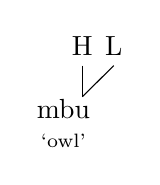
\begin{tikzpicture}[scale=.8]
			
			\node (seg) at (0,0) {mbu};
			\node[font=\scriptsize] at (0,-0.5) {`owl'};
			\node (H) at (0.3,1) {H};
			\node (L) at (0.8,1) {L};
			\coordinate (v) at (0.3,0.2);
			\draw (H.south) -- (v);
			\draw (L.south) -- (v);
		\end{tikzpicture}\hfil
		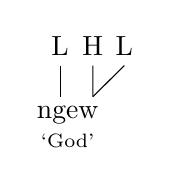
\begin{tikzpicture}[scale=.8]
	
			\node (seg) at (0,-.1) {ngew\textopeno\textopeno};
			\node[font=\scriptsize] at (0,-0.5) {`God'};
			
			\node (T1) at (-0.12,1) {L};
			\node (T2) at (0.4,1) {H};
			\node (T3) at (0.9,1) {L};
			
			\coordinate (a1) at (-0.12,0.2);
			\coordinate (a2) at ( 0.4,0.2);
			
			\draw (T1) -- (a1);
			\draw (T2) -- (a2);
			\draw (T3.south) -- (a2);
		\end{tikzpicture} \hfil
		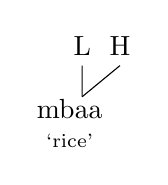
\begin{tikzpicture}[scale=.8]
			\node (c) at (0,0) {mbaa};
			\node[font=\scriptsize] at (0,-0.5) {`rice'};
			\node (t1) at (0.2,1) {L};
			\node (t2) at (0.8,1) {H};
			\draw (t1) -- (0.2,0.2);
			\draw (t2.south) -- (0.2,0.2);
		\end{tikzpicture} 
		&
		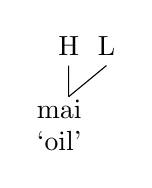
\begin{tikzpicture}[scale=.8]
			\node (c) at (0,0) {mai};
			\node (g) at (0,-0.5) {`oil'};
			\node (t1) at (0.15,1) {H};
			\node (t2) at (0.75,1) {L};
			\draw (t1) -- (0.15,0.2);
			\draw (t2.south) -- (0.15,0.2);
		\end{tikzpicture} \\ \midrule
		tone mapping 
		&
		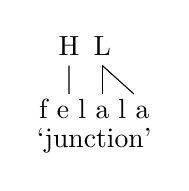
\begin{tikzpicture}[scale=.8]
			\node (c) at (0,0) {f e l a l a};
			\node (g) at (0,-0.5) {`junction'};
			\node (t1) at (-0.4,1) {H};
			\node (t2) at (0.13,1) {L};
			\draw (t1) -- ($(t1.south)+(0,-.45)$);
			\draw (t2) -- ($(t2.south)+(0,-.45)$);
			\draw (t2.south) -- ($(t2.south)+(.5,-.45)$);
		\end{tikzpicture} \hfil
		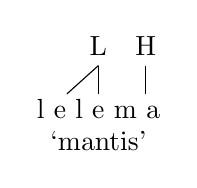
\begin{tikzpicture}[scale=.8]
			\node (c) at (0,0) {l e l e m a};
			\node (g) at (0,-0.5) {`mantis'};
			\node (t1) at (0,1) {L};
			\node (t2) at (0.75,1) {H};
			\draw (t1.south) -- ($(t1.south)+(0,-.45)$);
			\draw (t1.south) -- ($(t1.south)+(-.5,-.45)$);
			\draw (t2.south) -- ($(t2.south)+(0,-.45)$);
		\end{tikzpicture}
		&
		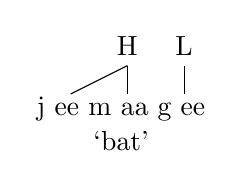
\begin{tikzpicture}[scale=.8]
			\node (c) at (0,0) {j ee m aa g ee};
			\node (g) at (0,-0.5) {`bat'};
			\node (t1) at (.1,1) {H};
			\node (t2) at (1,1) {L};
			\draw (t1.south)-- ($(t1.south)+(0,-.45)$);
			\draw (t1.south)-- ($(t1.south)+(-0.9,-.45)$);
			\draw (t2.south) -- ($(t2.south)+(0,-.45)$);
		\end{tikzpicture} \hfill
		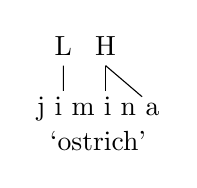
\begin{tikzpicture}[scale=.8]
			\node (c) at (0,0) {j i m i n a};
			\node (g) at (0,-0.5) {`ostrich'};
			\node (t1) at (-0.55,1) {L};
			\node (t2) at (0.12,1) {H};
			\draw (t1) -- ($(t1.south)+(0,-.4)$);
			\draw (t2.south) -- ($(t2.south)+(0,-.4)$);
			\draw (t2.south) -- (0.7,0.2);
		\end{tikzpicture}		\\ 
	\bottomrule
	\end{tabular}
	\caption{Contour inventories and tone mapping in Mende and Hausa.}
	\label{tab.hausa.mende}
\end{table}


There are mainly three approaches to the tone mapping problem. The
first identifies three key factors that determine the surface forms:
\textit{directionality} (whether tone spreads rightwards or leftwards), \textit{morphological categories }(prefix or suffix), and \textit{tone quality}
(whether spreading is sensitive to H or L) \citep{hyman1987prosodic,
	leben2017tone, hyman2009representation}.

The second account is Optimal Tone Mapping \citep[OTM;][]
{zoll2003optimal}. Zoll argues that directionality-based accounts of
phonological mapping can in some cases yield incorrect surface
predictions. Under OTM, surface tonal patterns emerge from
language-specific rankings between morphological faithfulness
constraints and markedness constraints, \textsc{Clash} and
\textsc{Lapse}, which are sensitive to tone quality.

The third approach, proposed by \citet{jardine2017LocalNature}, 
is to use language-specific, inviolable constraints, where the
constraints are marked, forbidden ARs; that is, ARs to be
avoided. For example, the \textsc{No Short Rise} constraint in Mende
\citep{leben2017tone} that bans monomoraic LH can be represented as a
banned AR as in Figure~\ref{graph:lh1}.

\begin{figure}[ht]
	\centering
	% --- Subfigure 1 ---
	\begin{minipage}[b]{0.25\textwidth}
		\centering
		\begin{tikzpicture}
			\node (neg) at (-0.8,2) {\Large $\neg$};		
			\node [] (t1) at (0,2) {L};
			\node [] (t2) at (0.6,2) {H};            
			\node [] (c1) at (0,1) {$\mu$};
			\node [] (s1) at (0,0) {$\sigma$};
			\draw [-] (t1) to (c1.north);
			\draw [-] (t2.south) to (c1.north);
			\draw (c1) -- (s1);
		\end{tikzpicture}
		\subcaption{*$\check{\mu}$}
		\label{graph:lh1}
	\end{minipage}
	\hfill
	% --- Subfigure 2 ---
	\begin{minipage}[b]{0.25\textwidth}
		\centering
		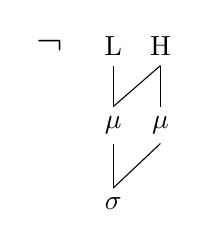
\begin{tikzpicture}
			\node (neg) at (-0.8,2) {\Large $\neg$};
			\node [] (t1) at (0,2) {L};
			\node [] (t2) at (0.6,2) {H};            
			\node [] (c1) at (0,1) {$\mu$};
			\node [] (c2) at (0.6,1) {$\mu$};
			\node [] (s1) at (0,0) {$\sigma$};
			\draw [-] (t1) to (c1.north);
			\draw [-] (t2.south) to (c1.north);
			\draw [-] (t2.south) to (c2.north);
			\draw [-] (c1.south) to (s1.north);
			\draw [-] (c2.south) to (s1.north);
		\end{tikzpicture}
		\subcaption{*$\check{\mu}\acute{\mu}$}
		\label{graph:lh2}
	\end{minipage}
	\hfill
	% --- Subfigure 3 ---
	\begin{minipage}[b]{0.3\textwidth}
		\centering
		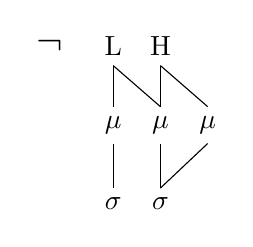
\begin{tikzpicture}
			\node (neg) at (-0.8,2) {\Large $\neg$};
			\node [] (t1) at (0,2) {L};
			\node [] (t2) at (0.6,2) {H};
			\node [] (c1) at (0,1) {$\mu$};
			\node [] (c2) at (0.6,1) {$\mu$};
			\node [] (c3) at (1.2,1) {$\mu$};
			\node [] (s1) at (0,0) {$\sigma$};
			\node [] (s2) at (0.6,0) {$\sigma$};
			\draw (t1.south) -- (c1.north);
			\draw (c1.south) -- (s1.north);
			\draw (t1.south) -- (c2.north);
			\draw (c2.south) -- (s2.north);
			\draw (t2.south) -- (c3.north);
			\draw (c3.south) -- (s2.north);
			\draw (t2.south) -- (c2.north);
		\end{tikzpicture}
		\subcaption{*$\grave{\mu}\check{\mu}\acute{\mu}$}
		\label{graph:lh3}
	\end{minipage}
	\hfill
\caption{The forbidden structure in (a), *$\check{\mu}$ (corresponding to \textsc{No Short Rise}), and two ARs in (b--c) containing it.}	\label{intro.fig.noLH}
\end{figure}

Following \citet{jardine2017LocalNature}, if
Figure~\ref{graph:lh1} is forbidden in the language, any AR
\textit{containing}~\ref{graph:lh1}, such as
\ref{graph:lh2} and \ref{graph:lh3}, will also be
forbidden. Formally, if Grammar $G$ is the set of constraints in the
language, such that \(G = \{AR_1, AR_2, \ldots, AR_n\}\), a well-formed
We represent factors as \emph{conjunctive negative literals}:
\(\lnot AR_1 \land \lnot AR_2 \land \ldots \land \lnot AR_n\)
\citep{jardine2017LocalNature,rogers.lambert2019mol}. It follows that
the tonotactic learning problem is to identify a set \(G\) of banned
ARs given a set of example surface forms. This paper follows the third
approach of \citet{jardine2017LocalNature}.  
%\input{sec1.fig.noLH.tex}

One potential criticism of \citet{jardine2017LocalNature}, anticipated
by the author and also applicable to the present work, is that it
explains tonal patterns exclusively in terms of surface-true
constraints. One consequence is that well-formed patterns that are not
directly observable in surface forms, or at the lexical level, are not
realised by the grammar. The grammar inferred at this level therefore
reflects only the final outcomes of tonal mapping, rather than
intermediate representations produced by tonal rules, which
potentially misses important phonological generalisations.
\hijeff{Do we want to mention ICGI paper here - maybe we should, why not}

Hausa provides a clear illustration of this point. The absence 
of rising tones on a single syllable can be explained as follows. 
An underlying LH sequence may arise as an intermediate representation, 
either through synchronic phonological processes or as the result of 
historical change, but it is subsequently simplified to either H in non-final 
position or L elsewhere \citep{Leben,Newmanbook}. Likewise, the absence of final 
L.L sequences on long vowels is attributed to \textsc{Low Tone Raising}, which 
changes underlying L.L to L.H when the second L occurs on a long vowel \citep{Leben,leben1996tonal}.
\hijeff{I removed the SPE styled rules and explained in prose instead.}

%\begin{multicols}{2}
%	\ea Rising Simplification \citep[p599]{Newmanbook}:\\
%	\noindent
%	LH $\rightarrow$ L / H \phold \\
%	LH $\rightarrow$ H / elsewhere
%	\z
%	\ea Low Tone Raising \citep{leben1996tonal}\\
%	\noindent
%	L [L, +long]  \# $\rightarrow$ L [H, +long]  \#\\
%	
%	\z
%\end{multicols}

This example illustrates that unattested surface patterns do not
necessarily reflect illicit structures in the grammar itself, but
rather intermediate representations that are subsequently subject to
some repair processes. While acknowledging the limitations of these
grammars, we argue that learning such grammars is nonetheless
valuable. They still provide meaningful insights into tonotactic
patterns and serve as a foundation for further work for three reasons.

First, a grammar containing a set of forbidden ARs that is consistent
with observable surface forms is not in conflict with a grammar for
the tonal processes; rather, it captures their pronounceable
outcomes. Given available access to a lexicon at a
different level of abstractness, another grammar could likewise be
learned, and these two grammars can be systematically compared. This
comparison between different levels of abstractness itself yields
non-trivial insights into tonal processes.

Second, considering that ARs have been long used in tonal phonology, 
yet absent from computational learning, we believe a more pressing 
priority is establishing representational adequacy for learning tones, 
which is the goal of this work.
Without an explicit framework
that encodes the geometry of tonal representations, modelling more
complex tonal alternations, such as those discussed above, is more
difficult. Establishing this representational foundation is therefore
a useful precondition for future work on deeper tonal processes.
\hijeff{On a second reading, I think this paragraph is still technically correct, but it now feels somewhat outdated. It reads like that we dont know whether transformations can be modeled over ARs, but we now know its possible, and exactly how do to}

Lastly, we are not aware of existing learning models that operate
with ARs directly for either tonal processes or tonotactics. In the next
section, we review previous learning approaches related to tier-based
representations and learning, and then introduce BUFIA, the algorithm
that our model is based on.

\subsection{Learning Models}\label{sec:learning.models}

This section reviews systems for phonotactic and tonotactic
learning. One line of research employs statistical methods from
machine learning \citep{CP97, hayes2008maximum,
	goldsmith2012information}. These methods have
been deployed on string and syllabic representations for learning
segmental phonotactic patterns as well as stress patterns,
but have not been used for learning tonotactics with ARs.

\citet{GouskovaGallagher2020} synthesises the Maximum Entropy (MaxEnt)
strategy of \citet{hayes2008maximum} with a procedure that induces
phonological tiers in order to learn non-local phonotactics. Related
work by
\citeauthor{Jardine-Heinz-2016-LTSLL}~(\citeyear{Jardine-Heinz-2016-LTSLL}),
\citeauthor{jardinemcmullin17}~(\citeyear{jardinemcmullin17}),
\citeauthor{de-santo-aksenova-2021-learning}~(\citeyear{de-santo-aksenova-2021-learning}),
and
\citeauthor{pmlr-v153-lambert21a}~(\citeyear{pmlr-v153-lambert21a}),
and \citeauthor{Swanson2025}~(\citeyear{Swanson2025}) provide
theoretical results and algorithms regarding the induction of
phonological tiers for non-local phonotactics. Other work has proposed
procedures for learning tiers for grammars modelling non-local
phonological processes \citep{BurnessMcMullin2019,
	burness-mcmullin-2021, Belth2024}. While the successful induction of
tiers from data is an important achievement of the 21st century, the
constraints induced over the projected tiers are still strings, and
not ARs. For example, none of the aforementioned methods can learn a
constraint that describes a many-to-one association from the tonal
tier to the TBU tier or vice versa.

BUFIA represents another approach \citep{chandleeBufia2019, rawski2021structure}.
BUFIA differs from the aforementioned approaches in a couple of ways. First,
it is not specific to any particular representation or data structure,
such as strings or trees. For this reason,
\citeauthor{chandleeBufia2019}'s (\citeyear{chandleeBufia2019})
presentation of BUFIA abstracts away from a specific representation,
and presents BUFIA in terms of arbitrary model-theoretic relational
structures. As long as the representations of interest can be
expressed model-theoretically, BUFIA can be implemented. %Consequently,
Since strings, trees, and graphs are all examples of structures that
have model-theoretic representations, versions of BUFIA can in
principle be designed for finding constraints over any of these
representations. This generality not only allows it to be
instantiated and ultimately deployed for the learning of a variety of
constraint types, but it also makes clear how the structure of the
space of possible constraints facilitates learning.

Second, BUFIA is a deterministic learning algorithm and in its current
form uses no statistical methods or randomness in its decision-making.
Basically, BUFIA checks possible constraints against the data one at a
time, adding those that are consistent with the data. It returns a
grammar consisting of inviolable constraints. As such, this grammar is
a conjunction of negative literals:
$\lnot C_1 \land \lnot C_2 \land \ldots \land \lnot C_n$, where each
\(C_i\) is a constraint, that is, a forbidden relational structure.

As will be explained in Section~\ref{sec:prelim.bufia}, BUFIA works because
any representational scheme orders the expressible constraints in a
natural way. By beginning with the smallest constraint, BUFIA is
guaranteed to search as much of the space as possible and return the
most general constraints (that is, the smallest forbidden structures)
consistent with the data, before a stopping condition is
met. Furthermore, BUFIA has been shown to be at least as successful in
learning feature-based, segmental phonotactics of Quechua
\citep{Swanson+2025} as phonotactic learning models based on the
principle of Maximum Entropy \citep{hayes2008maximum,
	wilson2018accidental}. However, BUFIA has not previously been used
in tonotactic learning over non-string representations.

To sum up, while ARs have long been conceptualised as graph
structures, no existing work learns grammars with ARs, nor has BUFIA
been instantiated to operate with ARs. To address this gap, we
present BUFIA-AR, a BUFIA-based learner capable of learning tonotactic
constraints directly over ARs. To our knowledge, BUFIA-AR is the first
learning algorithm that directly infers such constraints from ARs. As
an instantiation of the original BUFIA framework, BUFIA-AR inherits
its strengths and limitations.

A more detailed presentation of BUFIA-AR is given in Section~\ref{sec:bufiaar}. 
Before turning to that discussion, we first introduce in Section~\ref{sec:prelim} 
several elements from formal language theory, model theory, and graph theory that 
are essential for understanding the algorithm and its internal structure.  
Some of this background knowledge is well established in computer science 
\citep{CLRS2022,west2001introduction}; our presentation is adapted to suit those 
only familiar with phonological theory. 

\hijeff{I added the paragraph of math disclaimer back but
Im just worried that this is what R3 asked us to remove...}

We note that Section~\ref{sec:prelim} and ~\ref{sec:bufiaar} are
somewhat technical, and that researchers only interested in BUFIA-AR's
performance on the Hausa dataset may find them cumbersome. However, we
believe these sections are important to include because they provide
the necessary details for someone (1) to understand how BUFIA-AR is an
instantiation of the more general BUFIA algorithm, (2) to implement
the algorithm themselves (in order to replicate the study we
conducted), and (3) to understand how the algorithm's behaviour as well
as how it reflects the geometry of tonal phonology.

\section{Preliminaries} \label{sec:prelim} 

In this section, we begin with structures for representing strings
(Section~\ref{sec:prelim.string}), and then extend them to ARs using
graphs and matrices (Section~\ref{sec:prelim.ar}). Central to BUFIA is
Model Theory \citep{enderton2001mathematical}, which views structures
as mathematical objects, and uses formal logic to represent structural
units and the relationships between them. Model-theoretic analysis has
been used to compare differences between different representational
theories of phonological structure
\citep{strother-garciaUsingModelTheory,
	oakdenNotationalEquivalenceTonal2020, jardineetal20qtheoryAP}.  The
matrix-based representation used here is a common method in
mathematics and a particularly convenient way to represent AR
graphs. These formal representations are essential for subsequent
algorithm development, thereby understanding of the properties and
learnability of ARs.

\subsection{Strings Representations}\label{sec:prelim.string}
Tonal melodies can be represented as strings, that is, sequences of
symbols.  Let $\Sigma$ be a finite alphabet of symbols and $\Sigma^*$
the set of all strings over $\Sigma$. For example, in a language with
a tonal inventory $\{H, L\}$, we have $\Sigma = \{H, L\}$, and
$\Sigma^*$ contains all possible strings over $\Sigma$, such as
\textit{HL}, \textit{HHL}, \textit{HLHL}, and so on. Let $|w|$ 
denote the length of a string $w$. For $0 \le n < m \le |w|$,
let $w[n:m]$ denote a non-empty substring of $w$
starting at position $n$ and ending just before position $m$.
The empty string $\epsilon$ is trivially a substring of every string.

A string can also be represented \textit{model-theoretically} with two
components: the domain $D$ and a finite set of $n$-ary relations
$\mathcal{R} = \{ R_1, R_2, \ldots, R_i \}$ \citep{rogers2013,
	chandleeBufia2019, rogers.lambert2019mol}.  A string model of
\textit{HLHL} is shown in Figure~\ref{fig.model.str}.  In this
model, $D = \{1, 2, 3, 4\}$ indicates that there are four elements in
the string. Positions $\{1, 3\}$ are 
labelled with the unary relation $H$, while $\{2, 4\}$ are the
positions labelled with $L$.  Elements are connected via a
binary \textit{successor} relation, denoted by $\lhd$.  For example,
$\lhd = \{\langle 1, 2\rangle, \langle 2, 3\rangle, \langle 3,
4\rangle\}$ specifies that position 1 (labelled $H$) immediately
precedes position 2 (labelled $L$), position 2 immediately precedes
position 3, and so on.

\begin{figure}
	\centering	
	\begin{minipage}[r]{0.4\textwidth}
		\centering
		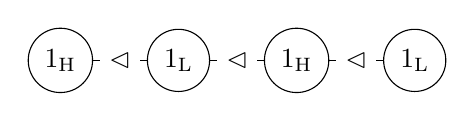
\begin{tikzpicture}[
			scale=.5,
			node distance=1.5cm,
			state/.style={draw,circle,minimum size=0.6cm}
			]
			\node[state] (1) {1\textsubscript{H}};
			\node[state,right of=1] (2) {1\textsubscript{L}};
			\node[state,right of=2] (3) {1\textsubscript{H}};
			\node[state,right of=3] (4) {1\textsubscript{L}};
			
			\draw (1) -- (2) node[midway,fill = white]  {$\lhd$};
			\draw (2) -- (3) node[midway,fill = white] {$\lhd$};
			\draw (3) -- (4) node[midway,fill = white] {$\lhd$};
			
%			\node[above=0.05cm of 1] {H};
%			\node[above=0.05cm of 2] {L};
%			\node[above=0.05cm of 3] {H};
%			\node[above=0.05cm of 4] {L};
		\end{tikzpicture}
	\end{minipage}
	\hfil
	\begin{minipage}[l]{0.40\textwidth}
		\small
		\[
		\begin{aligned}
			\mathcal{M} &= \{D \mid H,L,\lhd\} \\
			D           &= \{1,2,3,4\} \\
			H           &= \{1,3\} \\
			L           &= \{2,4\} \\
			\lhd        &= \{\langle1,2\rangle,\langle2,3\rangle,\langle3,4\rangle\}
		\end{aligned}
		\]
	\end{minipage}
	\caption{String model for \textit{HLHL} over $\Sigma=\{H,L\}$.}
	\label{fig.model.str}
\end{figure}

\subsection{Autosegmental Representation as Graphs}\label{sec:prelim.ar}

Unlike the string model, where elements are ordered linearly along a
single axis, an AR distributes linguistic information
across multiple tiers. In this work, in addition to the basic tone and
syllable tiers, we incorporate a mora tier, 
and treat the mora as a secondary unit subordinated
to syllables to indicate the syllable weight. Therefore,
we assume each syllable must associate with at least one
mora. %, with a pre-specified association line connecting them.
Figure~\ref{fig.model.AR1} illustrates a disyllabic form with an
LH.H melody, which is visualised as a graph in 
Figure~\ref{fig.model.AR2}, which corresponds to the model-theoretic 
relational structure in Figure~\ref{fig.model.AR3}.


\begin{figure}[ht]
	\centering
	% Autosegmental Representation
	\begin{minipage}[b]{0.2\textwidth}
		\centering
		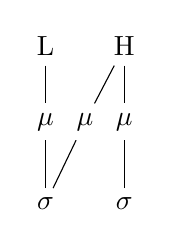
\begin{tikzpicture}
			\node (t1) at (1,1) {L};
			\node (t2) at (2,1) {H};
			
			\node[anchor=base] (c1) at (1,0) {$\mu$};
			\node[anchor=base] (c2) at (1.5,0) {$\mu$};
			\node[anchor=base] (c3) at (2,0) {$\mu$};
			
			\node (s1) at (1,-1) {$\sigma$};
			\node (s2) at (2,-1) {$\sigma$};
			
			\draw (t1) -- (c1);
			\draw (t2) -- (c2);
			\draw (t2) -- (c3);
			\draw (s1) -- (c1);
			\draw (s1) -- (c2);
			\draw (s2) -- (c3);            
		\end{tikzpicture} \vspace{2em}
		\subcaption{AR}
		
		\label{fig.model.AR1}
	\end{minipage}
	\hfill
	% Graph Representation
	\begin{minipage}[b]{0.4\textwidth}
		\centering
		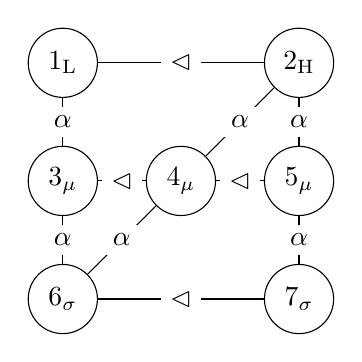
\begin{tikzpicture}[scale=0.5]
			\node[state] (t1) at (0,6) {1\textsubscript{L}};
			\node[state] (t2) at (6,6) {2\textsubscript{H}};
			
			\node[state] (c1) at (0,3) {3\textsubscript{$\mu$}};
			\node[state] (c2) at (3,3) {4\textsubscript{$\mu$}};
			\node[state] (c3) at (6,3) {5\textsubscript{$\mu$}};
			
			\node[state] (s1) at (0,0) {6\textsubscript{$\sigma$}};
			\node[state] (s2) at (6,0) {7\textsubscript{$\sigma$}};
			
			\draw (t1) -- node[midway, fill = white]  {$\alpha$} (c1) -- node[midway, fill = white] 
			{$\alpha$}(s1);
			\draw (t2) -- node[midway, fill = white]  {$\alpha$} (c2) -- node[midway, fill = white] 
			{$\alpha$}(s1);
			\draw (t2) -- node[midway, fill = white]  {$\alpha$} (c3) -- node[midway, fill = white] 
			{$\alpha$}(s2);
			
			
			\draw (t1) -- node[midway, fill = white] {$\lhd$} (t2);
			\draw (c1) -- node[midway, fill = white] {$\lhd$}(c2);
			\draw (c2) -- node[midway, fill = white] {$\lhd$}(c3);
			\draw (s1) -- node[midway, fill = white] {$\lhd$}(s2);
		\end{tikzpicture}
		\subcaption{Graph}
		\label{fig.model.AR2}
	\end{minipage}
	\hfill
	% Model Representation
	\begin{minipage}[b]{0.3\textwidth}
		\small
		\centering
		\begin{align*}
			%            M &= \langle D|  H, L, \mu, \sigma, \lhd, \alpha \rangle \\
			D &= \{1, 2, 3, 4, 5, 6, 7\} \\
			L &= \{1\}\\
			H &= \{2\}\\
			\mu &= \{3, 4, 5\}\\
			\sigma &= \{6, 7\} \\
			\lhd &= \{\, \langle 1,2 \rangle, \langle 3,4 \rangle, \langle 4,5 \rangle,
			\langle 6,7 \rangle\} \\
		\alpha &= \left\{
		\begin{aligned}
			&(1,3),(2,4),(2,5),\\
			&(3,6),(4,6),(5,7)
		\end{aligned}
		\right\}
		\end{align*}
		\subcaption{Model}
		\label{fig.model.AR3}
	\end{minipage}
	
	
	\caption{Three representations of a disyllabic LH.H}
	\label{fig.model.AR}
\end{figure}

A graph consists of a set of vertices $V$ and edges $E$.  
As can be seen in Figure~\ref{fig.model.AR3}, the graph consists
of seven \textit{labelled nodes} which are circles numbered with $\{1, 2,\dots,7\}$, 
representing linguistic units, each labelled with its corresponding properties, such
as $L$, $H$, $\sigma$, or $\mu$. 
The lines connecting elements are referred to as \textit{edges}, which 
may be either \textit{directed} or \textit{undirected}. For clarity, 
we distinguish two types of connections: \textit{association relations}, 
denoted by $\alpha$, refer to the undirected edges across tiers; 
%(e.g., between tones and moras, or between moras and syllables), 
and successor relations, denoted by $\lhd$, represent ordered relationships within a single tier. 
All the successor connections in the current example are given by
\( \lhd = \{\langle 1,2 \rangle,\ \langle 3,4 \rangle,\ \langle 4,5
\rangle,\ \langle 6,7 \rangle \}.\) The association relations, on the
other hand, are expressed as a set of unordered pairs:
\(\alpha = \{ (1,3),\ (2,4),\ (2,5),\ (3,6),\ (4,6),\ (5,7) \}.\)
Together, the tuple $\langle H, L, \mu, \sigma, \lhd, \alpha \rangle$
constitutes the \textit{signature} of this model-theoretic representation
of an AR.

In addition to representing model-theoretic relational structures 
with graphs, one can use \textit{adjacency matrices}
\citep{west2001introduction,CLRS2022}, which use binary values to
denote whether there is an edge between two nodes. Two nodes, $v$ and
$w$, are considered \textit{adjacent} if there is an edge connecting
them. If $G$ is a graph with $n$ nodes %,labelled $\{1, 2, \ldots, n\}$,
then its adjacency matrix $A$ is an $n \times n$ matrix. If $i$ and 
$j$ are connected, the entry $(i, j)$ has the value of 1; otherwise 
0. 
% As we will see, an adjacency matrix can be a
% useful tool for representing ARs. Since the nodes in ARs come from
% three disjoint sets (tones, moras, and syllables) and are connected by
% two levels of association edges (tone-to-mora and mora-to-syllable),
Using this method, an AR with $t$ tones, $m$ moras, and $s$ 
syllables can be encoded as a $t \times m$ tone-mora matrix and 
a $m \times s$ mora-syllable matrix, with successor relations 
implicit in the indexing. 
% A value of 1 indicates an association 
% between elements, and 0 indicates no association.
% \footnote{The matrix representation in computer science, where
	%   all nodes are encoded within a single adjacency matrix or a 
	%   three-dimensional matrix. This leverages the fact that all nodes 
	%   in an AR belong to three disjoint tiers, and that associations 
	%   occur only across tiers in particular ways. We also index rows 
	%   and columns of moras and syllables 
	%   for clarity which indices reflect temporal ordering.}

For instance, Table~\ref{tab.matrices} provides alternative
representation of the same AR in Figure~\ref{fig.model.AR}.
In the tone-mora matrix, the header row reflects the tonal sequence
$LH$, and the index column reflects the mora sequence. Since the L is
associated with the first mora $\mu_1$, and the H is associated with
both $\mu_2$ and $\mu_3$, the corresponding cells
$(L, \mu_1), (H, \mu_2), (H, \mu_3)$ are marked with 1, and others
with 0 which indicates no connection between them.\footnote{For
	convenience, we refer to each cell by the labels of the nodes. Node
	indices will be omitted from here on. For example, we may refer to $(1,3)$
	and $(2,4)$ with $(L,\mu_1)$ and $(H, \mu_2)$, respectively. However, 
	these are the labels of the nodes rather than the nodes 
	themselves.}  If we examine the matrix by columns, one can interpret that
the L tone occupies the first mora, while the H tone occupies the
remaining two.  Likewise, in the mora syllable matrix, since
$\sigma_1$ is associated with $\mu_1$ and $\mu_2$, and $\sigma_2$ with
$\mu_3$, the corresponding cells are marked with 1. If we examine this
matrix by rows, it can be seen that $\sigma_1$ is heavy while
$\sigma_2$ is light. Hereafter, we refer to the rows and columns in
the tone-mora matrix as the mora rows and tone columns respectively;
and to the rows and columns in the mora-syllable matrix as the
syllable rows and mora column respectively.
%
\begin{table}[ht]
	\centering
	\begin{tabular}{cc}
		% --- Column 1: Mora-Tone Matrix ---
		\(
		\begin{array}{c|cc}
			& L & H \\
			\hline
			\mu_1 & 1 & 0 \\
			\mu_2 & 0 & 1 \\
			\mu_3 & 0 & 1 \\
		\end{array}
		\)
		&
		% --- Column 2: Mora-Syllable Matrix ---
		\(
		\begin{array}{c|ccc}
			& \mu_1 & \mu_2 & \mu_3 \\ \hline
			\sigma_1 & 1     & 1     & 0     \\
			\sigma_2 & 0     & 0     & 1
		\end{array}
		\)
	\end{tabular}
	\caption{Adjacency matrices: tone–mora matrix (left) and mora–syllable matrix (right)}
	
	\label{tab.matrices}
\end{table}

These AR adjacency matrices capture precisely the same information as
the graphs and model-theoretic structures. If we replace the header
row and index column with the node numbers used in the graph model
signature, and replace the 1s with the indices of row and column, we
obtain the table filled as in Table~\ref{tab.index}. As can be
seen, these pairs are identical to the information encoded in
Figure~\ref{tab.matrices}
\hijeff{It might be more consistent/clear to replace the -> with \(\lhd\), as in the one on the left}

\begin{table}[ht]
	\centering
	\begin{tabular}{cc}
		$\begin{array}{c|c@{}c@{}c}
			& 1 & \lhd & 2 \\
			\hline
			3 & (1,3)  && 0 \\
			\bigtriangleup & && \\
			4 & 0 & & (2,4) \\
			\bigtriangleup & && \\
			5 & 0 & & (2,5) \\
		\end{array}$ &
		$\begin{array}{c|c@{}c@{}c@{}c@{}c}
			& 3 & \rightarrow & 4 & \rightarrow & 5 \\
			\hline
			6           & (3,6) &         & (4,6) &         &   	\\
			\downarrow  &       &         &       &         &   	\\
			7           &       &         &       &         & (5,7) \\
		\end{array}$
	\end{tabular}
\caption{Equivalent node-indexed encodings of the adjacency matrices in Table~\ref{tab.matrices}, where $\lhd$ and $\alpha$ are the successor and association predicates of the model signature.}
	\label{tab.index}
\end{table}

Furthermore, certain patterns can be easily identified by inspecting the
matrices. For example, a series of contiguous 1s may indicate tone 
spreading over multiple moras if observed in the tone column, or a mora 
shared by multiple tones if seen in the mora row. 
Two 1s positioned diagonally suggest a one-to-one mapping.
The associations $(L,\mu_1)$ and $(H,\mu_2)$
in the tone-mora matrix in Table \ref{tab.matrices}
present an example of this.
Some particular or ill-formed patterns can also be 
readily detected, which will be discussed in Section~\ref{sec:bufiaar}.

\subsection{Structure Containment}
%
An important concept when considering model-theoretic relational
structures, either strings, sequences of feature bundles, or ARs, is
\textit{containment}. Intuitively, containment refers to the situation
when one structure includes another structure inside of it. We
formalise this notion using two related definitions, following
\citet{chandleeBufia2019}: \textit{restriction}
(Definition~\ref{def.res}) and \textit{containment}
(Definition~\ref{def.contain}). Readers are referred to
\citet{rogers.lambert2019mol} for an alternative formulation. In the
definitions below, it is assumed the structures A and B have the same
signature $\langle R_1, \ldots R_n \rangle$.

\begin{definition}
	\label{def.res}
	\textit{ $A= \langle D^A; R^A_1, \ldots, R^A_n \rangle$ is a \emph{restriction}
		of $B
		= \langle D^B; R^B_1, \ldots, R^B_n \rangle$ iff $D^A \subseteq D^B$ and for
		each $m$-ary relation $R^A_i$, we have $R^A_i = \{(x_1, \ldots, x_m) \in R^B_i \mid x_1, \ldots, x_m \in D^A\}$. }
\end{definition}

\begin{definition}
	\label{def.contain}
	\textit{Structure $A$ is \emph{contained} in structure $B$
		($A \sqsubseteq B$) if there exists a restriction of $B$, denoted
		$B'$, and there exists a function $h:A \rightarrow B'$ such that for
		each $m$-ary relation $R_i$ in the model signature:
		\(R_i(a_1, \ldots, a_m) \in A \implies R(h(a_1), \ldots, h(a_m)) \in
		B'.\)}
\end{definition}

These definitions mean that $A$ is \textit{contained} in $B$ whenever
there exists a subpart of $B$ onto which \(A\) projects via a function
\(h\), and furthermore, that the relations that hold among elements of
\(A\) hold among their corresponding elements in \(B\). For instance,
the AR in Figure~\kuo{sec3.fig.restriction:a} is contained in the AR
in \kuo{sec3.fig.restriction:b} because the dotted region in
\kuo{sec3.fig.restriction:b} preserves all internal relations of
%:
\kuo{sec3.fig.restriction:a}, despite the differences in the
indicing. In particular, $\mu_1, \mu_2, \sigma_1$ in
\kuo{sec3.fig.restriction:a} project to $\mu_2, \mu_3, \sigma_2$ in
\kuo{sec3.fig.restriction:b}, respectively.

%\input{sec3.fig.restriction}

The containment relation is particularly important because it provides
a natural \textit{ordering} over the space of possible structures. The
ordering is not total, like a linear order; it is a \textit{partial}
ordering. In such a partially-ordered space, some structures are
comparable in terms of containment, but not necessarily all of them
are. \citet{chandleeBufia2019} provides some additional terminology:
if one structure \(A\) is contained in another structure \(B\), then
structure \(A\) is a \textit{subfactor} of structure \(B\), whereas
\(B\) is a \textit{superfactor} of \(A\). They prefer these terms to
substructures and superstructures, which have different
technical meanings in model theory.

To illustrate, Figure~\ref{fig.hasse.str} displays a
non-exhaustive portion of the partial ordering of possible strings
over the alphabet $\Sigma = \{a,b\}$. At the bottom of the ordering is
the empty string $\epsilon$, with more complex strings appearing
higher in the ordering.  Whenever two elements are connected by a
line, it means the higher element contains the lower element. For
example, no line relates the \(a\) to \(b\), because neither contains
the other.  However, a line is drawn from \(a\) to \(aa, ab\) and
\(ba\), because \(a\) is contained in each of these structures. As
defined above, \(aa, ab, ba\) and \(aaa\), and any other strings that
contain \(a\) are superfactors of \(a\); correspondingly, \(a\) is a
subfactor of each of these strings.

There can be many layers between a superfactor and one of its 
subfactors. When there are no structures ordered between a 
superfactor and its subfactor, it is called a \textit{next superfactor}. 
In this sense, among all superfactors of \(a\) such as 
\(\{aa, ab, ba, aaa, aab, \cdots\}\), only those superfactors that 
are exactly one level above are next superfactors of \(a\), 
namely \(\{aa, ab, ba\}\).

\begin{figure}
	\centering
	\begin{tikzpicture}[
		every node/.style={inner sep=1pt, font=\small\itshape},
		edge/.style={},
		]
		\matrix (m) [matrix of nodes,
		row sep=6mm,
		column sep=10mm,
		nodes={anchor=center},
		]{
			\node (aaa) {aaa}; &\node (llb1) {...};&   \node (llb2) {...}; & \node (llb3) {...};&\node (llb4) {...};&\node (llb5) {...};&    \node (bbb) {bbb}; \\
			&\node (aa) {aa}; & \node (ab) {ab}; && \node (ba) {ba}; & \node (bb) {bb}; \\
			&& \node (a) {a}; & & \node (b) {b}; &  \\
			&&& \node (z) {$\epsilon$}; && \\};
		
		\draw[edge] (z) -- (a);
		
		\draw[edge] (z) -- (b);
		
		\draw[edge] (a) -- (aa) -- (aaa);
		\draw[edge] (a) -- (ab);
		\draw[edge] (a) -- (ba);
		
		\draw[edge] (b) -- (bb) -- (bbb);
		\draw[edge] (b) -- (ab);
		\draw[edge] (b) -- (ba);
		\draw[edge, dotted] (aa) -- ++(0,1.5em);
		%	\draw[edge, dotted] (aa) -- ++(1,1.5em);
		\draw[edge, dotted] (ab) -- ++(0,1.5em);
		%	\draw[edge, dotted] (ab) -- ++(1,1.5em);	
		%	\draw[edge, dotted] (bb) -- ++(-1,1.5em);	
		\draw[edge, dotted] (ba) -- ++(0,1.5em);
		\draw[edge, dotted] (bb) -- ++(0,1.5em);
	\end{tikzpicture}
	\caption{Strings over $\Sigma = \{a,b\}$ ordered by the containment relation (non-exhaustive)}
	\label{fig.hasse.str}
\end{figure}%



\begin{Backmatter}

\paragraph{Competing interests}

The authors declare that there are no conflicts of interest regarding the publication of
this paper.


\paragraph{Acknowledgments}
We would like to thank John Goldsmith for his careful reading of earlier drafts and 
for his many insightful comments and suggestions. We also benefited from 
discussions with the audiences of the Stony Brook PhoRum, Rutgers Subregular 
Workshop, including Ellen Broselow, Thomas Graf, Jiwon 
Yun, and Adam Jardine. Finally, the detailed and constructive feedback from three 
anonymous reviewers, the Editor, the Associate Editor greatly improved strengthened 
both analysis and the presentation in this paper.

\paragraph{Funding statement}
This research was supported by grants from the <funder-name><doi>(<award ID>); <funder-name><doi>(<award ID>).

\paragraph{Data availability statement}
A statement about how to access data, code and other materials allowing users to understand, verify and replicate findings --- e.g. Replication data and code can be found in Harvard Dataverse: \url{https://doi.org/link}.

\paragraph{Ethical standards}
The research meets all ethical guidelines, including adherence to the legal requirements of the study country.

\paragraph{Author contributions}
A.A. and A.B.C. designed the study, abstracted the data wrote the first draft, and approved the final
version of the manuscript. A.R.E.J., M.R.L., K.L.S., and A.D.P. revised the manuscript and approved the final version.

\paragraph{Supplementary material}
State whether any supplementary material intended for publication has been provided with the submission.

\bibliography{ref.bib}
\bibliographystyle{apalike}

\end{Backmatter}
\end{document}
